

%----------------------------------------------------------------------------------------
%	PACKAGES AND DOCUMENT CONFIGURATIONS
%----------------------------------------------------------------------------------------

\documentclass[a4paper,12pt]{article}
\usepackage{siunitx} % Provides the \SI{}{} and \si{} command for typesetting SI units
\usepackage{graphicx} % Required for the inclusion of images
\usepackage{subfigure}
\usepackage{multirow}
\usepackage{amsmath} % Required for some math elements 
\usepackage{indentfirst}
\usepackage{times} % Uncomment to use the Times New Roman font
\usepackage{appendix}
\usepackage{verbatim}

%----------------------------------------------------------------------------------------
%	DOCUMENT INFORMATION
%----------------------------------------------------------------------------------------

\title{ \rule{\textwidth}{0.3mm} \\UM–SJTU JOINT INSTITUTE \\ PHYSICS LABORATORY \\ (VP141) \\ \rule{\textwidth}{0.3mm} \\ [30 mm]  \Large{Laboratory Report} \\[5 mm]  Exercise 4 \\[1 mm] Measurement of the Speed of Sound\\[15 mm]} % Title
\author{Cao Zhiyuan} % Author name
\date{\today} % Date for the report

\begin{document}
\scshape

\maketitle % Insert the title, author and date

\begin{center}
\begin{tabular}{l l l}
\\[6 mm]
%Date Performed: & June 22, 2019  \\
Partners:  \\
Name: Cao Zhiyuan & ID: 518370910030 & Group: 14 \\
Name: Ouyang Wenbing & ID: 518021910945 & Group: 8 \\
~\\
Date Performed:\\
June 21, 2019\\
\end{tabular}
\end{center}

\thispagestyle{empty}


\newpage


\small\tableofcontents
\thispagestyle{empty}


\newpage

%----------------------------------------------------------------------------------------
%	SECTION 1
%----------------------------------------------------------------------------------------

\setcounter{page}{1}
\upshape
\section{\textsc{Introduction}}
\subsection{\textsc{Theoretical Background}}
Sound, as one of the commonest way to convey message, plays an indispensable part in our daily life. In fact, sound wave is a mechanical wave which is generated from a vibration source. In order that the wave propagates, some compressible medium is needed, which also act as a parameter influencing the speed of sound. If classified from the aspect of propagation direction, sound is a longitudinal wave whose displacement is in the same direction to its propagation. For human beings, they can only hear the sound with frequency ranging from 20 Hz to 20,000 Hz. If the frequency is larger than 20,000 Hz, then it is called \textsl{ultrasound}. In our experiment, taking into consideration the condition in a teaching laboratory, we choose ultrasound as the signal source for its wavelength is appropriately short enough for us to observe.\par
The phase speed \textit{v}, at which the speed of the phase propagates, can be related to frequency \textit{f} and wavelength \textit{$\lambda$} though the following formula:

\begin{equation} \label{eq1}
\textit{$v=\lambda f$} 
\end{equation}

Besides, if an object moves along a straight line with its distance travelled \textit{L} and time used \textit{t} known, its phase speed can be calculated through the following formula accordingly:

\begin{equation} \label{eq2}
\textit{$v = \frac{L}{t} $}
\end{equation}

\subsection{\textsc{Measurement Methods}}
\subsubsection{\textsc{Resonance Method}}
For resonance method, we have wave source \textit{$S_1$} and receiver \textit{$S_2$} (which can be also called receiver) whose distance from each other is \textit{L}. In the situation where they are parallel to each other, it should satisfy the following format to form a standing wave:

\begin{equation}
\textit{$L=n\frac{\lambda}{2}~~(n = 1,2,3,...)$}
\end{equation}

From Eq.(3), the standing wave form if and only if the distance between the wave source \textit{$S_1$} and receiver \textit{$S_2$} is about half of the wavelength. By observing the horizontal difference between the peak of wave (See Fig.1), half of the wavelength \textit{$\frac{\lambda}{2}$} is easy to find, and then, with the frequency \textit{f} read directly from the signal generator, plug them in Eq.(1), the speed of sound \textit{v} can be calculated accordingly. 

\begin{figure}[h] 
    \centering
    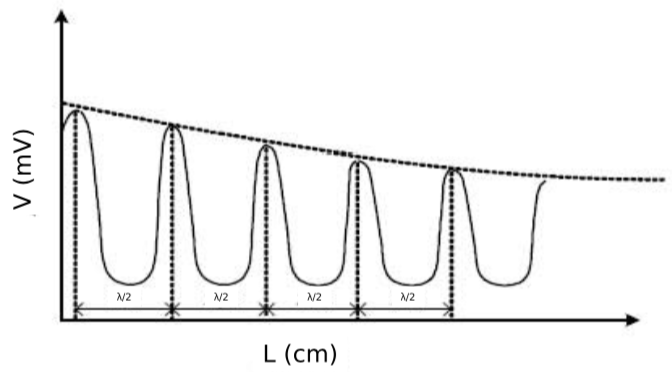
\includegraphics[width=0.5\textwidth]{Fig1} 
    \caption{Relationship between voltage and distance between the transducers \cite{labmanual}} 
\end{figure}

\newpage

\subsubsection{\textsc{Phase-comparison Method}}
In terms of Phase-comparison method, from the theoretical background, if in the propagation direction two waves have the same phase, then the distance between them must be divisible by its wavelength \textit{$\lambda$}. In other words, the following equation always holds:

\begin{equation}
\textit{$L = n \lambda~~(n = 1,2,3,...)$}
\end{equation}

\begin{figure}[htbp]
\centering
\subfigure[$\omega = 1~\&~\delta = 0$]{
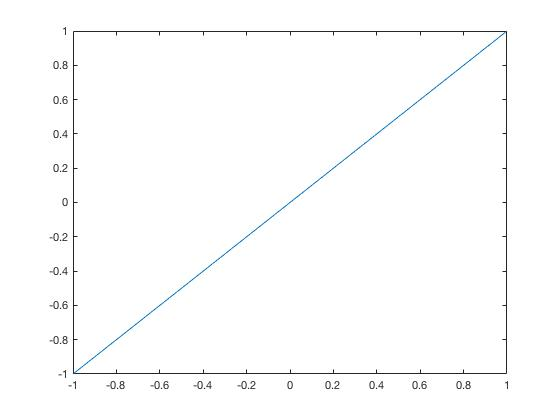
\includegraphics[width=5.5cm]{Fig2}
%\caption{fig1}
}
\quad
\subfigure[$\omega = 1~\&~\delta = \frac{\pi}{4}$]{
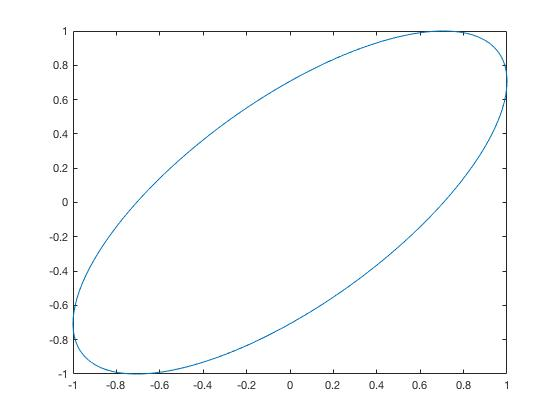
\includegraphics[width=5.5cm]{Fig3}
}
\quad
\subfigure[$\omega = 1~\&~\delta = \frac{\pi}{2}$]{
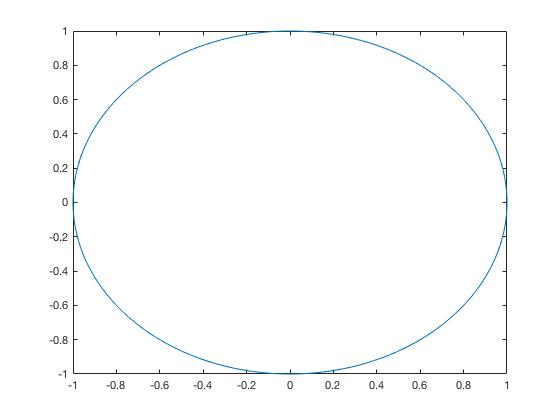
\includegraphics[width=5.5cm]{Fig4}
}
\quad
\subfigure[$\omega = 1~\&~\delta = \pi$]{
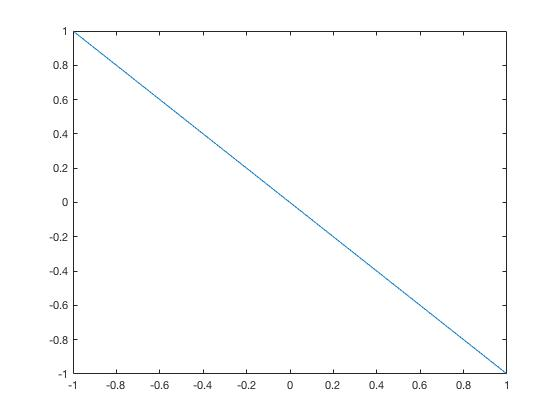
\includegraphics[width=5.5cm]{Fig5}
}
\caption{Lissajous figures of \textit{x}~=~sin(\textit{$\omega$}t~+~$\delta$) and  \textit{y}~=~sin(\textit{$\omega$}t) w.r.t. different $\delta$}
\end{figure}

\newpage

In order to identify the specific value of \textit{L}, Lissajous figures are used in this method. According to the definition, Lissajous figures are "the trajectories of a particle moving simultaneously in two perpendicular directions (for example, the axes x and y of a Cartesian coordinate system), so that the motion along each axis is simple harmonic (with different natural angular frequencies, amplitudes and initial phases, in general)"\cite{labmanual}. To be more specific, for parametric equations \textit{x}~=~sin(\textit{$\omega$}t~+~$\delta$) and  \textit{y}~=~sin(\textit{$\omega$}t), the shape of the trajectory changes with respect to $\delta$ (See Fig.2). Particularly, when $\delta$ = 2\textit{n}$\pi$~(n = 0,1,2,3,...), the shape of the cure is a straight line with a positive slope. Hence the wavelength \textit{$\lambda$} can be calculated accordingly.

\subsubsection{\textsc{Time-difference Method}}
When an ultrasonic signal is emitted by generator \textit{$S_1$} and received by \textit{$S_2$}, it is reflected back to \textit{$S_1$}. Hence the travelling time \textit{$\Delta t$} can be shown on the oscilloscope. Then, the distance \textit{L} can be read directly from the ruler. By plugging in \textit{$\Delta t$} and \textit{L} into Eq.(2), the phase speed of sound is obtained eventually.

%----------------------------------------------------------------------------------------
%	SECTION 2
%----------------------------------------------------------------------------------------

\section{\textsc{Apparatus and Experimental Setup}}
For this experiment, the apparatuses used are a signal source, two piezoelectric transducers \textit{$S_1$} and \textit{$S_2$}, and oscilloscope \cite{labmanual}.

\begin{figure}[h] 
    \centering
    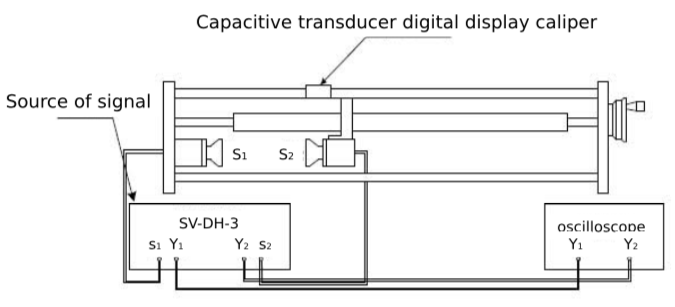
\includegraphics[width=1\textwidth]{Fig6} 
    \caption{The experimental setup \cite{labmanual}} 
\end{figure}

The oscilloscope is a device transforming the electric signals into visible messages which can be easily analyzed by humans. In this experiment, we use oscilloscope to figure out the state of our waves. \par
The two piezoelectric transducers \textit{$S_1$} and \textit{$S_2$} are connected to a ruler which has a precision of 0.001[mm]. Thus data with high accuracy is more likely to be obtained.\par
To begin our experiment, we first connect signal source, piezoelectric transducers and oscilloscope together as shown in Fig.1. Then, we adjust the frequency and mode of the oscilloscope to prepare it for our experiment.\par
To see the detailed parameters of each apparatus, see the following table:

\begin{table}[h]
\begin{tabular}{ccc}
\hline
Name of the instrument & Measured quantities & Precision / Type-B Uncertainty\\
\hline
Thermometer & Temperature & $\pm 1[^{\circ}C]$\\
Callipers & Distance & $\pm 0.001 [mm]$\\
Oscilloscope & Frequency & $\pm 0.001 [kHz]$\\
& Time & $\pm 0.2 [\mu s]$\\
\hline
\end{tabular}
\caption{Table of details in the Instruments}
\end{table}

%----------------------------------------------------------------------------------------
%	SECTION 3
%----------------------------------------------------------------------------------------
\section{\textsc{Measurements}}
\subsection{\textsc{Procedures \cite{labmanual}}}
\subsubsection{\textsc{Resonance Method}}
\begin{itemize}
\item[1.]
Set the initial distance of \textit{$S_1$} and \textit{$S_2$} at approximately 10[mm].
\item[2.]
Turn on the oscilloscope, and then warm it up by doing the following procedures:
	\begin{itemize}
	\item[(1)] 
	Select the wave type to be sine (continuous).
	\item[(2)]
	Switch the Signal Strength so that the voltage reaches peak on oscilloscope.
	\item[(3)]
	Find the optimal frequency ranging from $34.5[kHz]$ to $40[kHz]$ so that the voltage have its maximum value on the screen. Then record the frequency.
	\end{itemize}
\item[3.]
By increasing the distance $L$ between \textit{$S_2$} and \textit{$S_1$}, the output voltage function on the oscilloscope changes its shape. Find the particular distance $L$ so that the voltage's amplitude reaches its peak. Record the value $L$.
\item[4.]
Do step 3 for 10 more times to record 12 values of $L$. Then, do a linear fit to find out the slope, which is half of the wavelength. 
\end{itemize}
\subsubsection{\textsc{Phase-comparison Method}}
\begin{itemize}
\item[1.] 
According to what has been illustrated in Introduction, Lissajous figures helps determine the wavelength. Record the distance $L$ between \textit{$S_1$} and \textit{$S_2$} when the figure becomes a straight line with a positive slope.
\item[2.]
Repeat step 1 until we get 12 values to perform a linear fit. 
\end{itemize}
\subsubsection{\textsc{Time-difference Method}}
\begin{itemize}
\item[1.] 
Switch the medium to water.
\item[2.]
Alter the frequency of wave to 100 Hz and width with 500 $\mu$s.
\item[3.]
Push the CURSOR button on the oscilloscope to measure the time the sound travels and the corresponding distance. Record 12 pairs of data so that a linear fit can be performed to find out $v_{sound}$.
\end{itemize}
\subsection{\textsc{comments/observations regarding the measurements}}
\begin{itemize}
\item[1.]
Note that when moving the piezoelectric transducers, their distance from each other should not be less than $10 mm$. Otherwise their will be some magnetic actions happening among them, which will not only cause damage on the instruments, but influence the accuracy of experiment data as well.
\item[2.]
While reading the values on callipers, the last digit should be estimated, which may result in some instability of the accuracy.
\item[3.]
During the process of experimenting, make sure that the callipers moves in one direction and cannot moves back. Otherwise some accuracy will occur because of backslash error.
\item[4.]
When doing the "Phase-comparison method" part, we should estimate whether the curve turns into a line with positive slope. Therefore, instability of reading may happen if the "decision" of whether the trajectory has already been a straight line differs. To minimize the error, the judgement ought to be accomplished by a single person so that the "feeling" always keep the same.
\item[5.]
Remember not to splash the water on the callipers in case that the calliper rusts and the calibration changes.
\end{itemize}

%----------------------------------------------------------------------------------------
%	SECTION 4
%----------------------------------------------------------------------------------------

\section{\textsc{Results}}
\subsection{\textsc{Resonance Method}}
By reading the value on the oscilloscope, we obtain the frequency of the sound wave is:

\begin{center}
$f = 36.638 [kHz] \pm 0.001 [kHz]$
\end{center}

Then, from the thermometer, we obtain the temperature is:

\begin{center}
$T = 22[^{\circ}C] \pm 1[^{\circ}C]$
\end{center}

The following table shows the distance between \textit{$S_1$} and \textit{$S_2$} when the amplitude of the wave reaches its peak successively. 

\begin{table}[h]
\begin{center}
\begin{tabular}{|c|c||c|c|}
\hline
\multicolumn{2}{|c||}{$L_i[mm] \pm 0.001[mm]$} & \multicolumn{2}{c|}{$L_i[mm] \pm 0.001[mm]$}\\
\hline
1 & 28.671 & 7 & 57.372 \\
2 & 33.448 & 8 & 62.035 \\
3 & 38.220 & 9 & 66.788 \\
4 & 42.996 & 10 & 71.548 \\
5 & 47.815 & 11 & 76.295 \\
6 & 52.553 & 12 & 81.027 \\
\hline
\end{tabular}
\caption{Data table for Resonance Method}
\end{center}
\end{table}

Hence, we are able to further plot the linear fit figure, whose slope is half of the wavelength, with the help of \textit{sciDAVis}. The L-i linear fit plot is shown in the following figure: \par

\begin{figure}[h] 
    \centering
    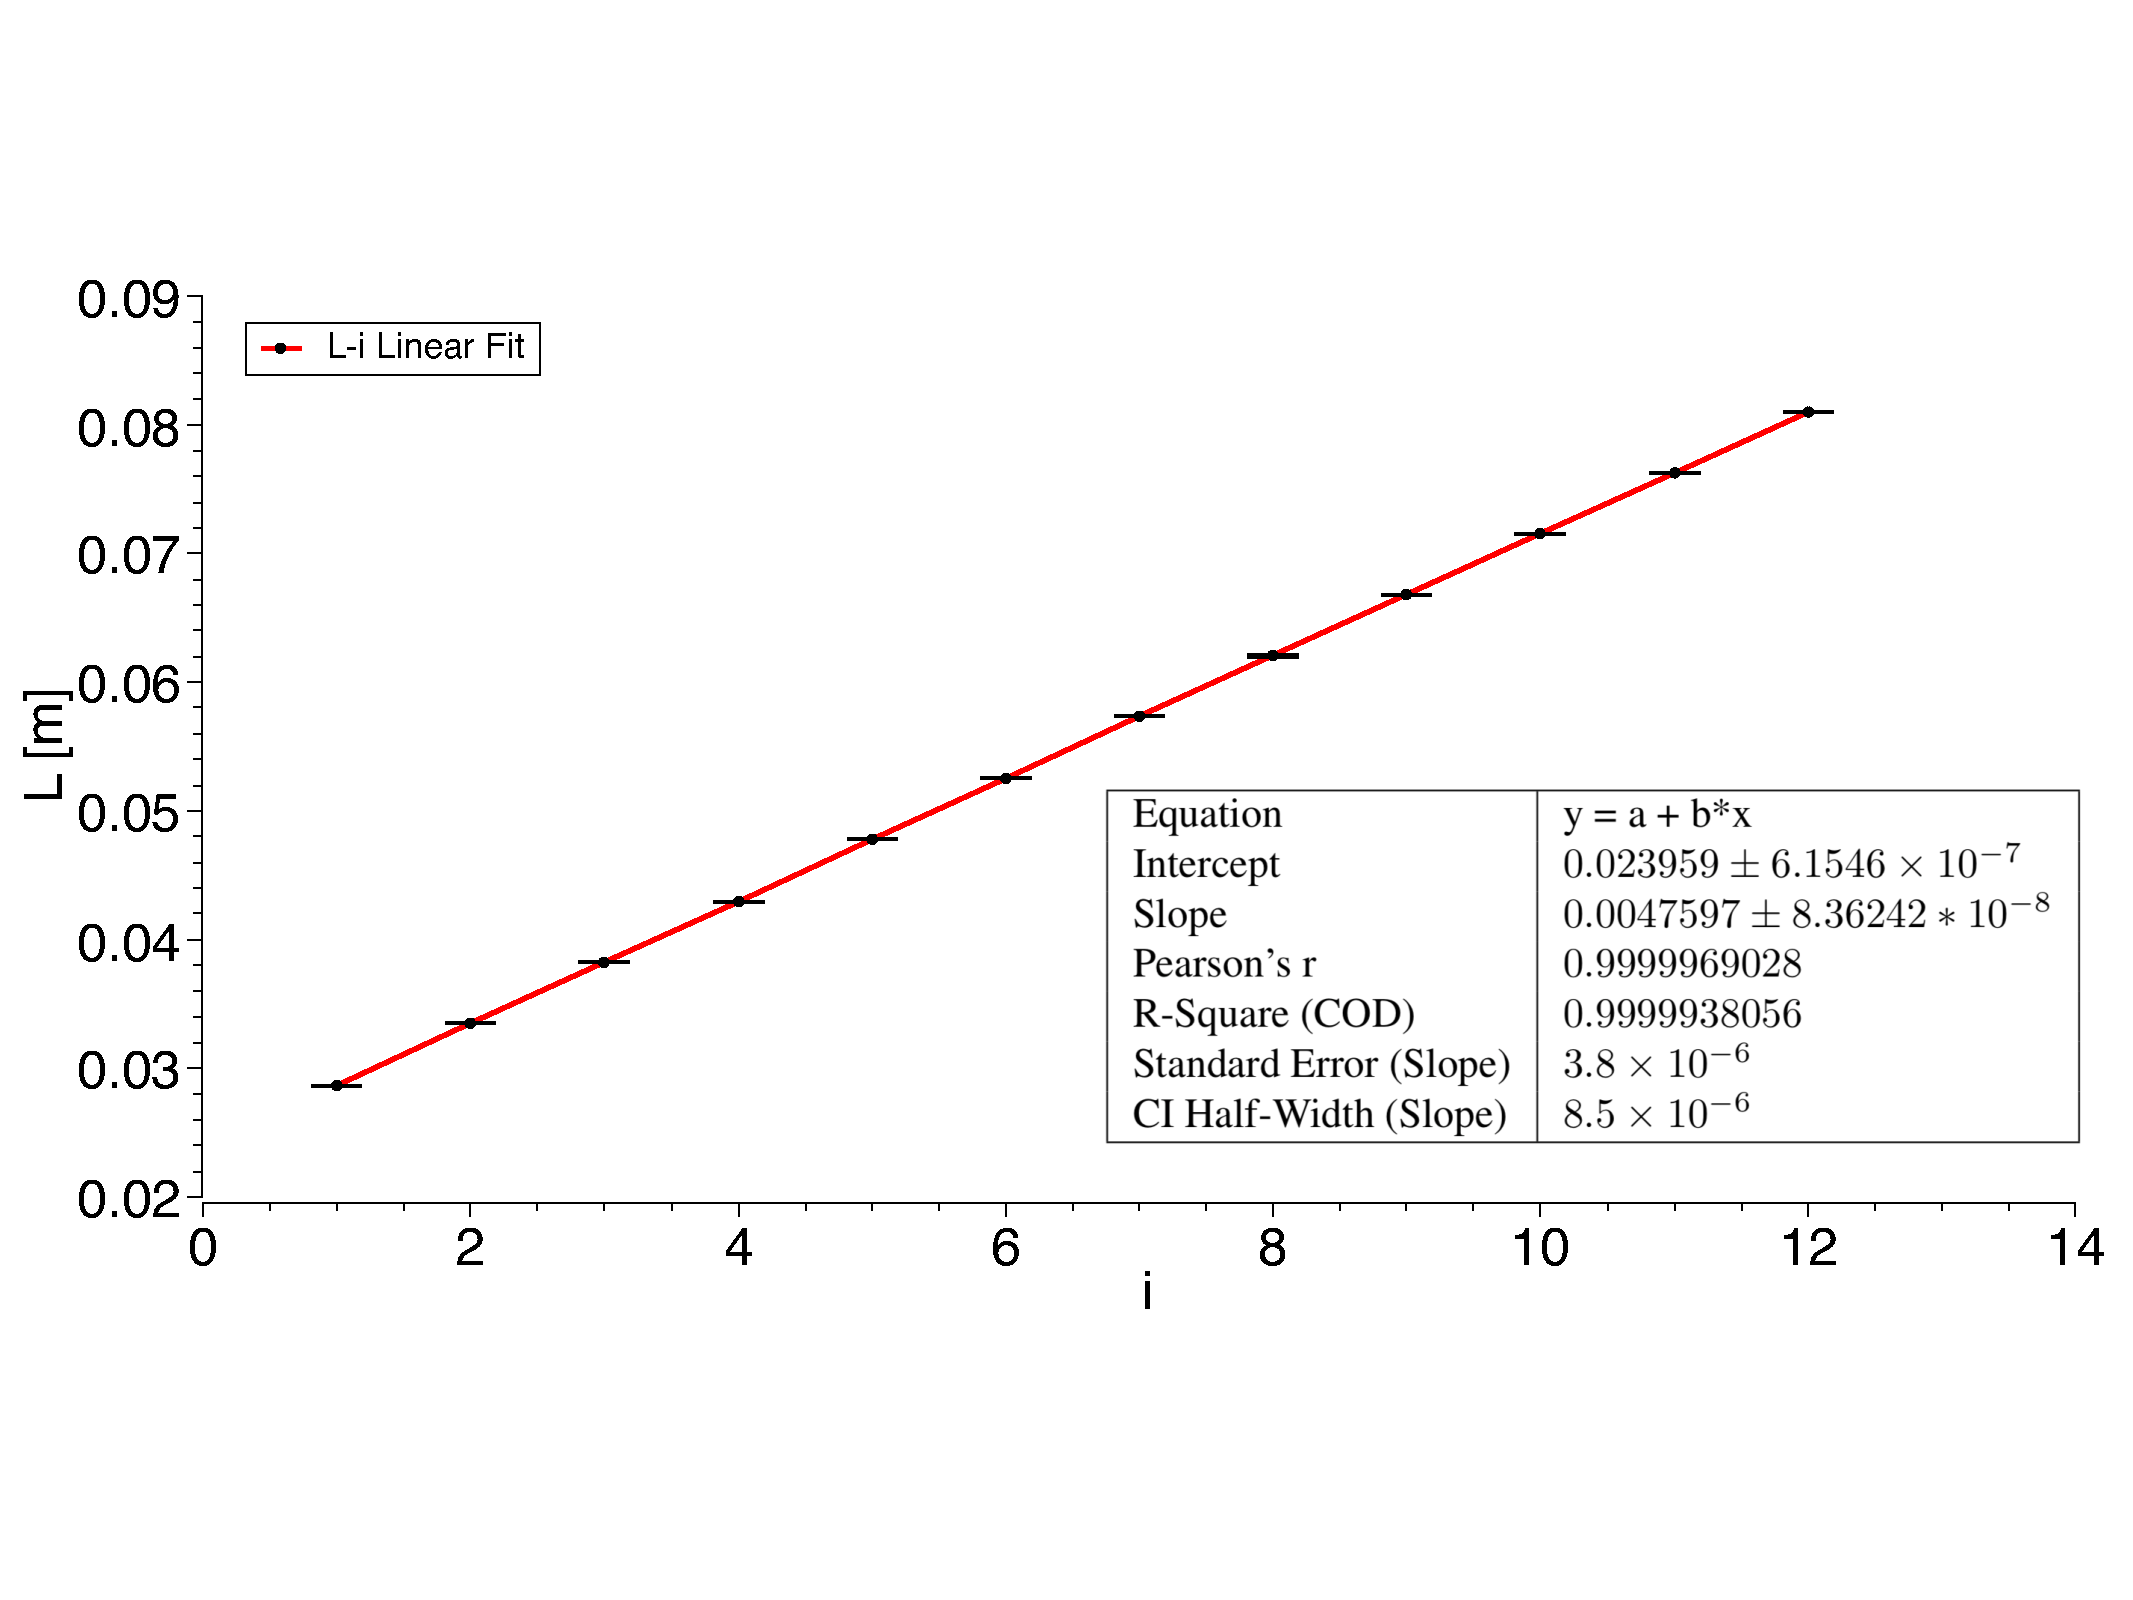
\includegraphics[width=1.04\textwidth]{Fig7_2} 
    \caption{Linear Fit figure for L-i in Resonance Method} 
\end{figure}

\begin{comment}
\begin{table}[h]
\begin{center}
\begin{tabular}{|l|l|}
\hline
Equation & y = a + b*x \\
Intercept & $ 0.023959 \pm 6.1546 \times 10^{-7}$ \\
Slope & $ 0.0047597 \pm 8.36242*10^{-8}$ \\
Pearson's r & $0.9999969028$ \\
R-Square (COD) & $0.9999938056$ \\
Standard Error (Slope) & $3.8 \times 10^{-6}$ \\
CI Half-Width (Slope) & $8.5 \times 10^{-6}$ \\
\hline
\end{tabular}
\caption{Detailed parameters for the L-i Linear Fit}
\end{center}
\end{table}
\end{comment}

Hence, according to Eq.(1), the speed of sound can be found as:

\begin{center}
$ v = \lambda f = 348.772 \pm 0.623~[m/s]$
\end{center}

with relative uncertainty $ 0.179\% $. (The detailed calculations are shown in Appendix A.2.1)

\subsection{\textsc{Phase Comparison Method}}
The wave frequency we used and temperature remain the same as we used in Resonance Method, namely:

\begin{center}
$f = 36.638 [kHz] \pm 0.001 [kHz]$\\
[3 mm]
$T = 22[^{\circ}C] \pm 1[^{\circ}C]$
\end{center}

The following table is obtained by recording the distance between \textit{$S_1$} and \textit{$S_2$} when the Lissajous figure has the shape of a straight line with a positive slope.

\begin{table}[h]
\begin{center}
\begin{tabular}{|c|c||c|c|}
\hline
\multicolumn{2}{|c||}{$L_i[mm] \pm 0.001[mm]$} & \multicolumn{2}{c|}{$L_i[mm] \pm 0.001[mm]$}\\
\hline
1 & 111.528 & 7 & 168.812 \\
2 & 121.440 & 8 & 178.525 \\
3 & 131.377 & 9 & 188.613 \\
4 & 140.805 & 10 & 198.440 \\
5 & 150.170 & 11 & 207.780 \\
6 & 159.089 & 12 & 216.989 \\
\hline
\end{tabular}
\caption{Data table for Phase Comparison Method}
\end{center}
\end{table}

Hence, we are able to further plot the linear fit figure, whose slope is the wavelength, with the help of \textit{sciDAVis}. The L-i linear fit plot is shown in the following figure:

\begin{figure}[h] 
    \centering
    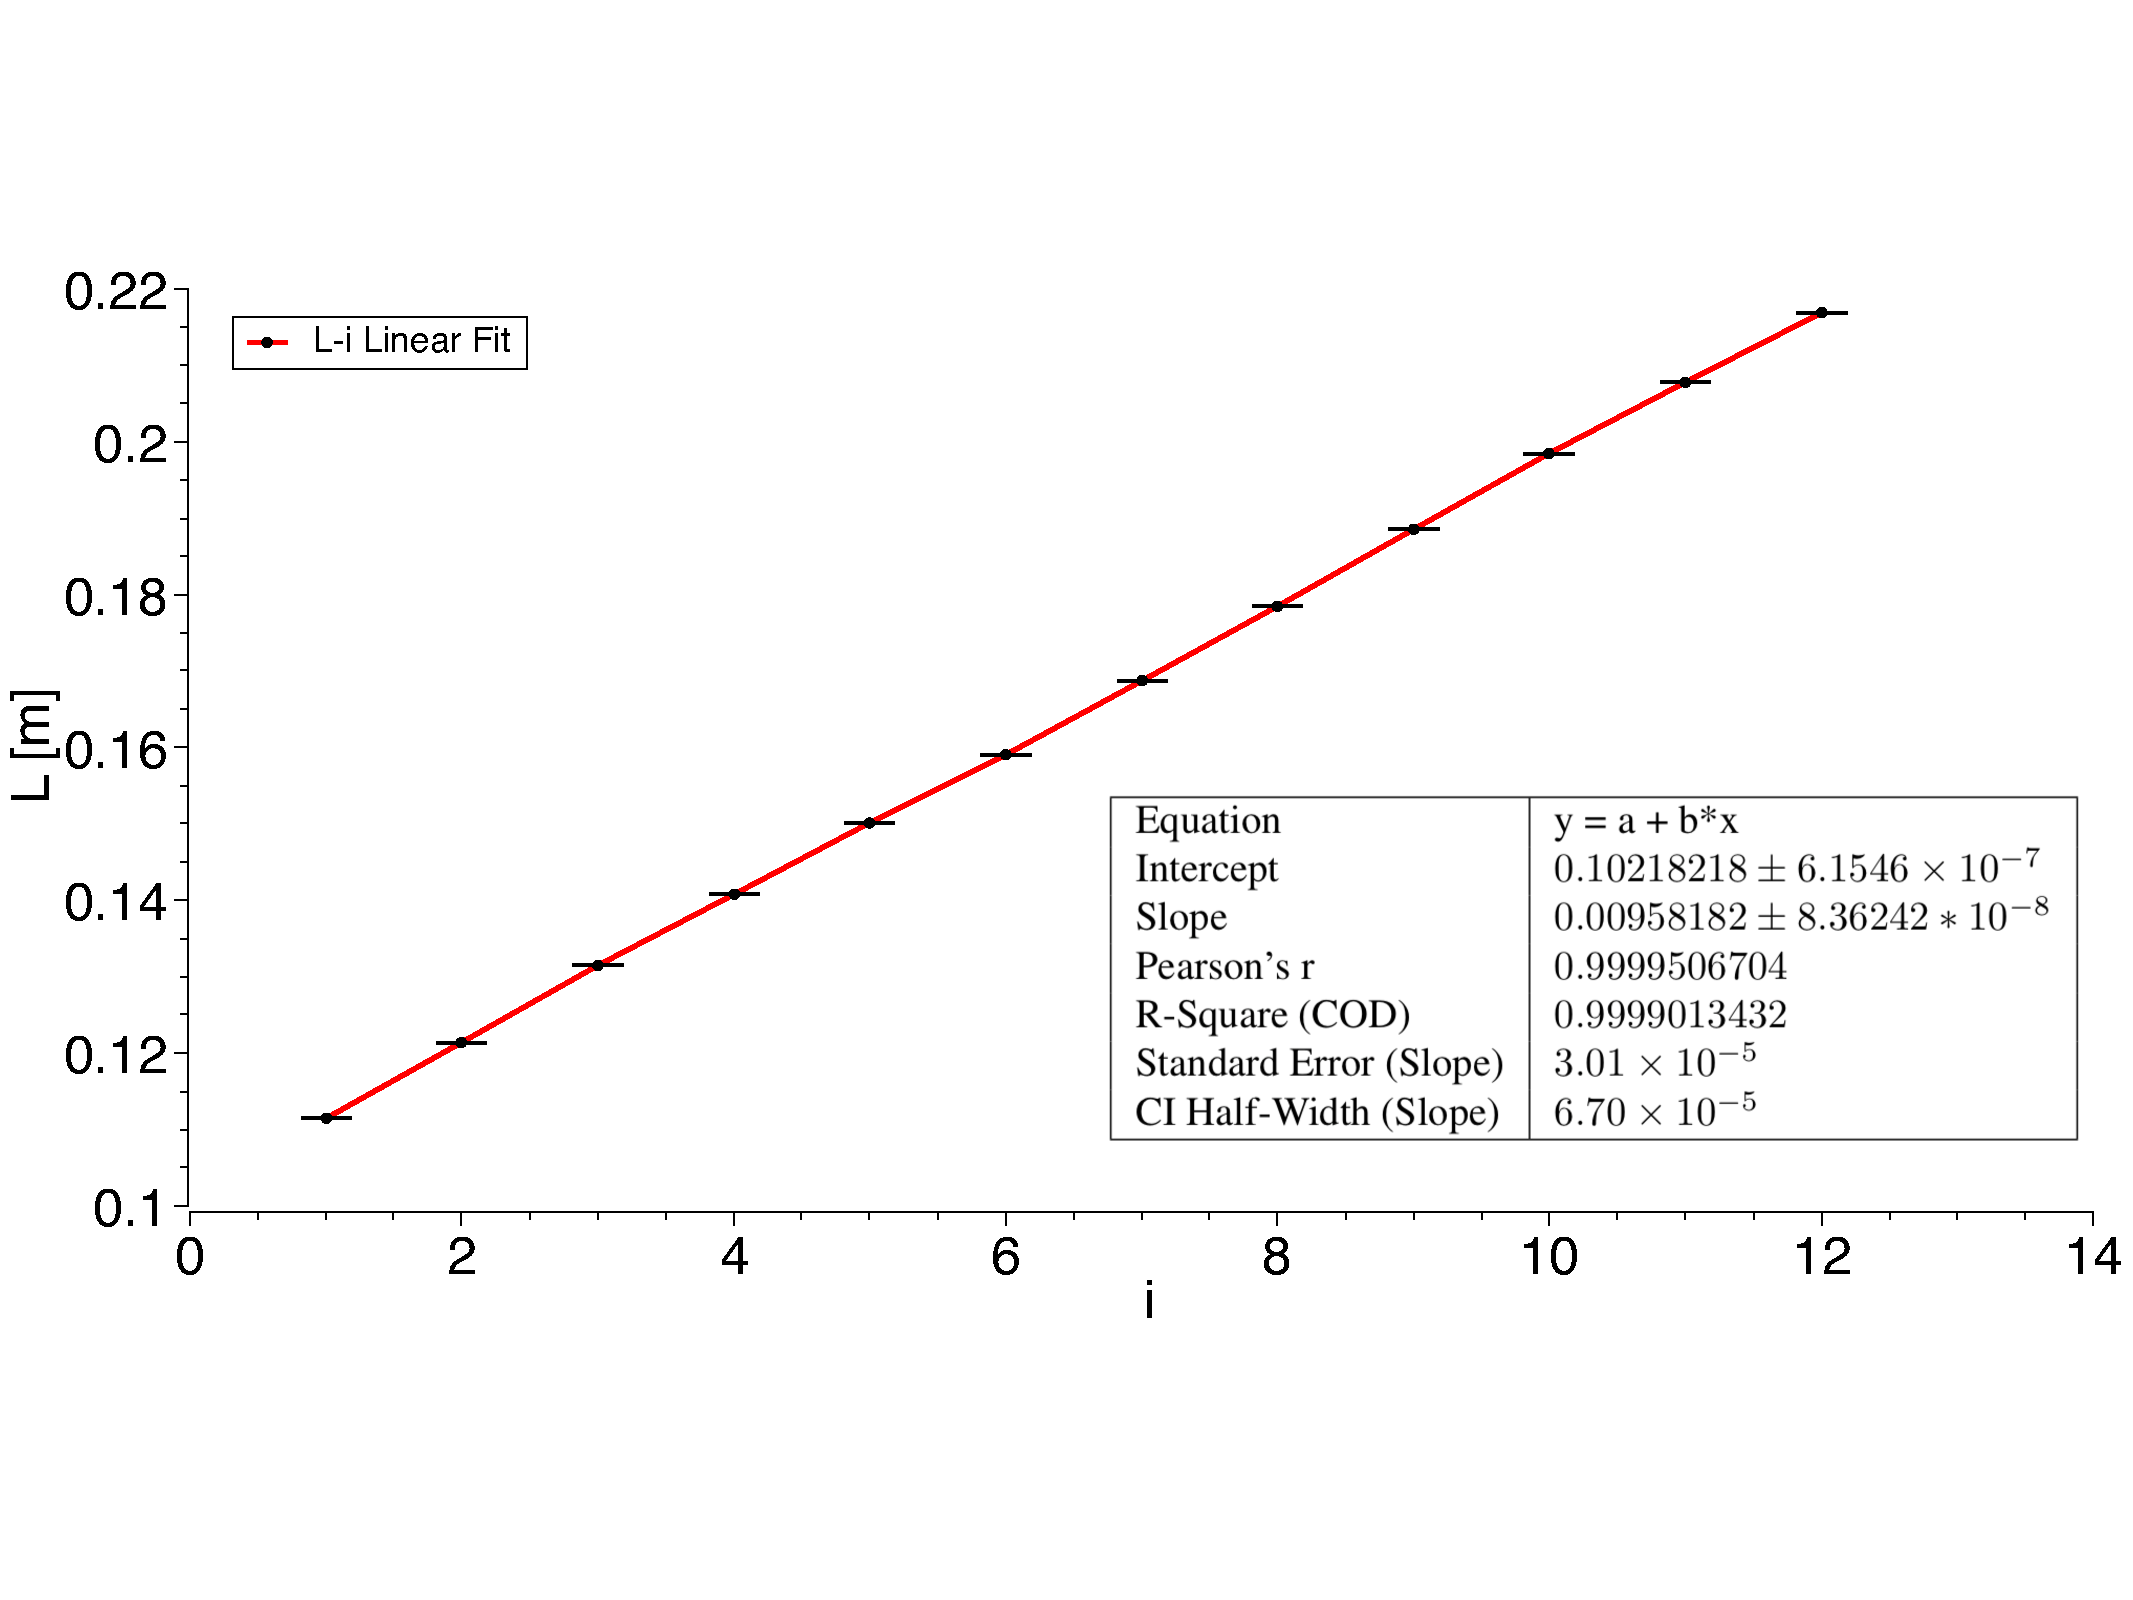
\includegraphics[width=1.04\textwidth]{Fig8_2} 
    \caption{Linear Fit figure for L-i in Phase Comparison Method} 
\end{figure}

\begin{comment}
\begin{table}[h]
\begin{center}
\begin{tabular}{|l|l|}
\hline
Equation & y = a + b*x \\
Intercept & $0.10218218 \pm 6.1546 \times 10^{-7}$ \\
Slope & $0.00958182 \pm 8.36242*10^{-8}$ \\
Pearson's r & $0.9999506704$ \\
R-Square (COD) & $0.9999013432$ \\
Standard Error (Slope) & $3.01 \times 10^{-5}$ \\
CI Half-Width (Slope) & $6.70 \times 10^{-5}$ \\
\hline
\end{tabular}
\caption{Detailed parameters for the L-i Linear Fit}
\end{center}
\end{table}
\end{comment}

\newpage

Hence, according to Eq.(1), the speed of sound can be found as:

\begin{center}
$ v = \lambda f = 351.059 \pm 2.455~[m/s]$
\end{center}

with relative uncertainty $ 0.699\% $. (The detailed calculations are shown in Appendix A.2.2)


\subsection{\textsc{Time Difference Method}}

In time difference method, we have the distance $L_i$ the sound travelled and the corresponding time $ t $. Then, we apply a linear fit to find out the speed of sound. The data collected are shown in the following table.

\begin{table}[h]
\begin{center}
\begin{tabular}{|c|c|c|}
\hline
  & ~~~~~$t_i[\mu s] \pm 0.2[\mu s]$~~~~~ & $L_i[mm] \pm 0.001[mm]$ \\
\hline
1 & 109.2 & 150.862 \\
2 & 112.6 & 155.670 \\
3 & 115.8 & 160.462 \\
4 & 119.4 & 165.558 \\
5 & 122.8 & 170.490 \\
6 & 126.2 & 175.882 \\
7 & 129.6 & 180.582 \\
8 & 132.8 & 185.541 \\
9 & 136.0 & 190.581 \\
10 & 139.6 & 195.650 \\
11 & 143.0 & 220.525 \\
12 & 146.4 & 205.560 \\
\hline
\end{tabular}
\caption{Data table for Time Difference Method}
\end{center}
\end{table}

Then, we perform the t-L linear fit and obtain the figure below.


\begin{figure}[h] 
    \centering
    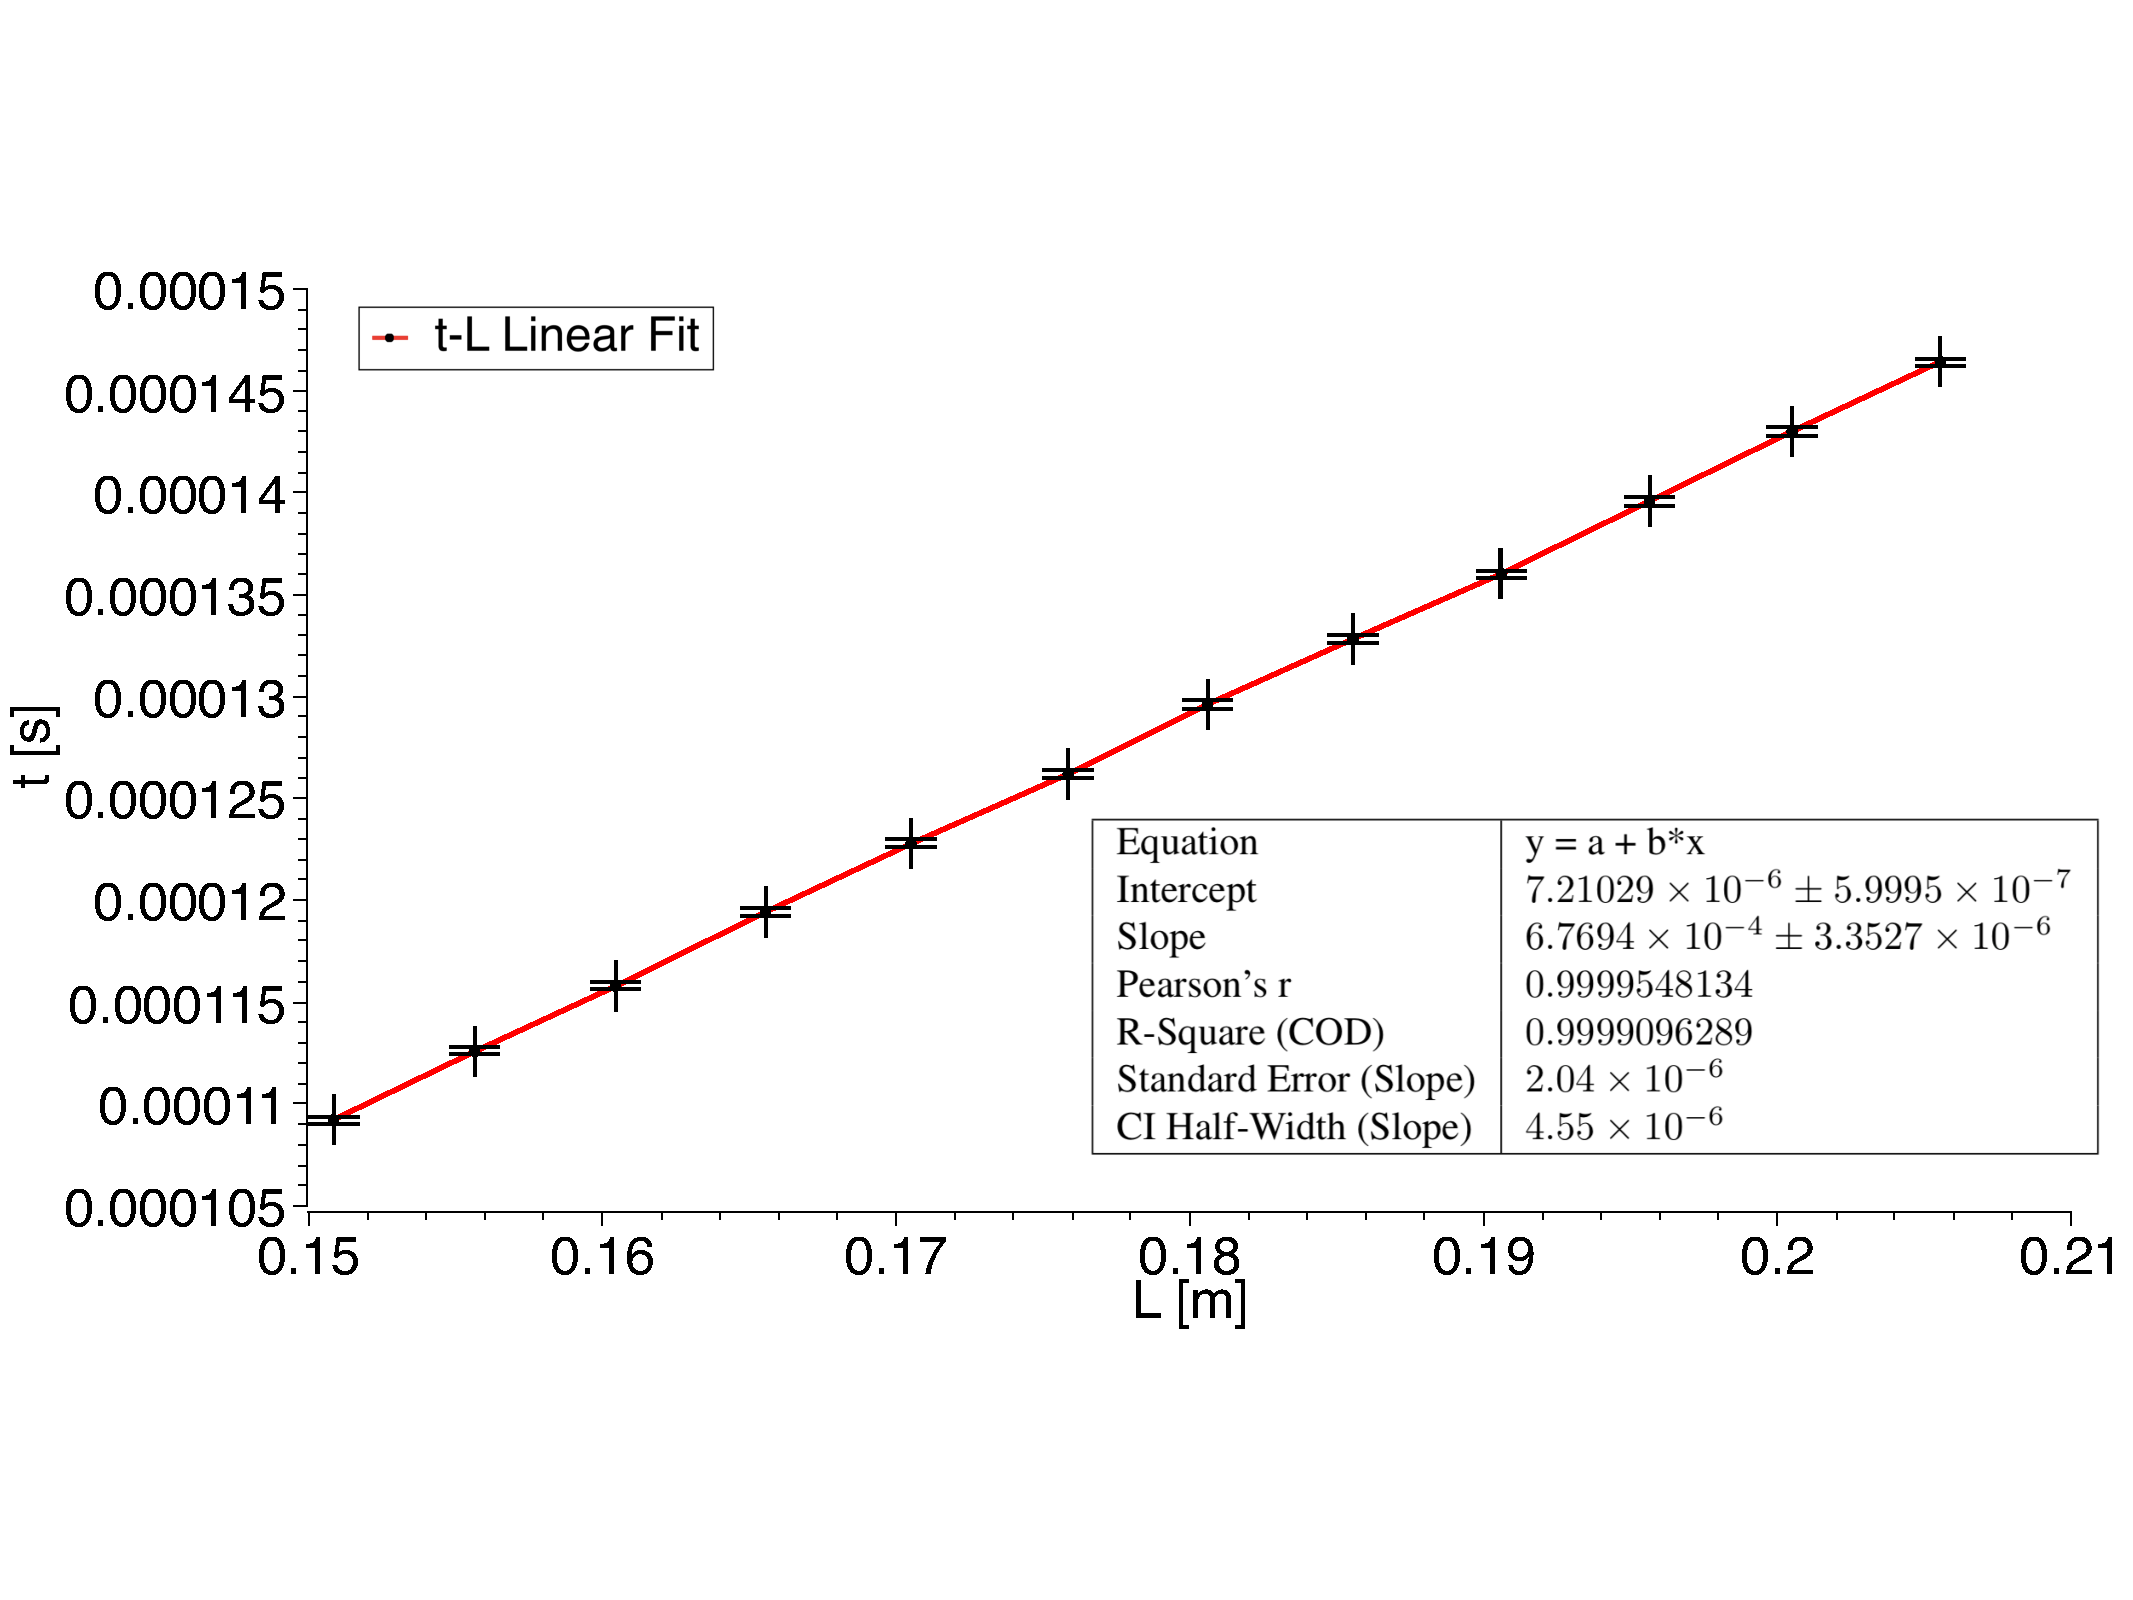
\includegraphics[width=1.04\textwidth]{Fig9_2} 
    \caption{Linear Fit figure for L-i in Time Difference Method} 
\end{figure}

\begin{comment}
\begin{table}[h]
\begin{center}
\begin{tabular}{|l|l|}
\hline
Equation & y = a + b*x \\
Intercept & $7.21029 \times 10^{-6} \pm 5.9995 \times 10^{-7}$ \\
Slope & $6.7694 \times 10^{-4} \pm 3.3527 \times 10^{-6}$ \\
Pearson's r & $0.9999548134$ \\
R-Square (COD) & $0.9999096289$ \\
Standard Error (Slope) & $2.04 \times 10^{-6}$ \\
CI Half-Width (Slope) & $4.55 \times 10^{-6}$ \\
\hline
\end{tabular}
\caption{Detailed parameters for the t-L Linear Fit}
\end{center}
\end{table}
\end{comment}

\newpage

Therefore, since the slope of it equals to 1/$v$, we can obtain the speed of sound:

\begin{center}
$\displaystyle v = \frac{1}{k_3} \approx 1477.236 \pm 9.929 [m/s]$
\end{center}

with relative uncertainty $ 0.672\% $. (The detailed calculations are shown in Appendix A.2.3)

%----------------------------------------------------------------------------------------
%	SECTION 5
%----------------------------------------------------------------------------------------

\section{\textsc{Conclusion and Discussion}}
\subsection{\textsc{Discussion about the results and error analysis}}
In our experiment, the speed of sound in air is found by measuring the wavelength and frequency and then multiply them together. Resonance Method and Phase Comparison Method yield the values
\begin{center}
$v = 348.772 \pm 0.623~[m/s]$ ~and~ $v = 351.059 \pm 2.455~[m/s]$
\end{center}
respectively. According to the estimated value in \textit{The Physics Factbook} \cite{ct1}, the speed of sound in 22 $^{\circ}C$ is $v = 344.7 \pm 0.6 [m/s]$. Our measured data is higher than expected, with a relative difference $1.18\%$ and $1.84\%$. \par
The most obvious source of experimental uncertainty comes from the judgement of figure. Since the accuracy of instruments has already been high enough, what makes the value inaccurate may derive from human issues, i.e. whether the Lissajous figures have turned into a straight line or it's still a ellipse. While in the boundary situation, it's hard for us to judge accurately. Hence errors may occur. \par 
Besides, taking into consideration that both the values measured in Resonance Method and Phase Comparison Method are higher than estimated, chances are that there are some deviations while using the thermometer to measure temperature. The temperature might be higher than 22 $^{\circ}C$: it may change slightly while we are doing the experiments, which is possibly the reason why the values of speed are somewhat higher.\\
 \par
Speaking of our speed of sound in water, which is found by Time Difference Method with a linear fit, our calculated value is 
\begin{center}
$v = 1477.226 \pm 9.929 [m/s]$
\end{center}
According to \textit{The Physics Factbook} \cite{ct1}, the speed of sound in water ranges from $1450 [m/s]$ to $1498 [m/s]$ depending on the characteristics of water. The experiment value (taking into consideration the uncertainty) confirms the theoretical value cited. The source of inaccuracy may be the reading error from the callipers and oscilloscope or the quality of water (in terms of density, temperature, viscosity, etc.). 

\subsection{\textsc{Some important cautions regarding the experiment}}
\begin{itemize}
\item[(1)] Why we need to measure Temperature T [$^{\circ}C$]? \par
The surrounding temperature act as an indispensable factor influencing the speed of sound regardless of whether the medium is air or water. Though the quantity influence of temperature can't be easily obtained, the general trend is that the speed of sound increase with the elevation of temperature. Since the influence isn't negligible, we should record the temperature as a parameter.
\item[(2)] In Phase-Comparison Method, why we use straight line Lissajous figures as reference? \par
The major reason why we choose straight line as reference is that it can be easily recognized by humans. Consider if we choose a circle or ellipse as a reference, will it be possible for us to make a precise judgement for 12 times? Hence, choosing straight line as reference can enhance the accuracy of our data, which leads to a lower uncertainty. To make our slope be the exact value of wavelength, we decide to choose a straight line with positive slope as reference.
\item[(3)] In Time Difference Method ,why we choose $L_0 > 100~[mm]$?\par 
If the distance between the piezoelectric transducers are less or equal to $100~[mm]$, there may be some magnetic actions happening between them, which will not only cause damage on the instrument, but influence the accuracy of data as well. 
\end{itemize}

\subsection{\textsc{Some possible improvements}}
In the experiment, some improvements may help increase the accuracy of measurements.
\begin{itemize}
\item[(1)] When using the oscilloscope in Resonance Method and Phase Comparison Method, we should slow up adjusting the distance if our figure is approaching the critical state (e.g., the Lissajous Figures has the trend to become a straight line in Phase Comparison Method). In this way we are more likely to obtain a relative accurate data.
\item[(2)] To further explore the influence of temperature on the speed of sound, we can measure the sound speed at different $T$ to understand to what extent temperature will influence our measurements.
\item[(3)] During experiment,instability of reading may happen if the ”decision” of whether the trajectory has already been a critical state differs. To minimize the error, the judgement ought to be accomplished by a single person so that the ”feeling” always keep the same.
\end{itemize}
%----------------------------------------------------------------------------------------
%	SECTION 6
%----------------------------------------------------------------------------------------

\begin{appendices} 
      \section{\textsc{Measurement uncertainty analysis}} 
      \subsection{\textsc{Uncertainty of single measurements}}
      In this experiment, we performed single measurements due to the following reasons:
      \begin{itemize}
      \item[a)] 
      The precision of the experiment is high enough so that there is no need to do multiple measurements: The precision has reached as high as $0.001 [mm],~0.001 [kHz],$ etc.
      \item[b)]
      Because the time spent on doing one experiment is relatively too long, we choose not to repeat the experiment several times.
      \item[c)]
      For some measurements the apparatus yields the same result throughout the experiment. For instance, the thermometer's value won't change by multi-measurements. 
      \end{itemize}
      \par
      In the case of single measurements, there is no \textit{Type-A Uncertainty}. Hence, the uncertainties are taken as:
      		\begin{equation}
      		u_{single} = \sqrt{\Delta_A^2 + \Delta_B^2} = \Delta_B = \Delta_{dev}
      		\end{equation}
      		\par
      In our experiment, we use the following quantities which have single measurements uncertainties. The particular uncertainties are recorded below.
      \subsubsection{\textsc{Uncertainty of measurement of temperature}}
      Since the temperature is measured by thermometer directly only once, the uncertainty is simply $\Delta_{dev}$. Hence, the uncertainty is $u_{Tem}~ = 1[^{\circ}C]$.
       \subsubsection{\textsc{Uncertainty of measurement of distance}}
      Since the distance is measured by callipers directly only once, the uncertainty is simply $\Delta_{dev}$. Hence, the uncertainty is $u_D = 0.001 [mm] = 1 \times 10^{-6} [m]$.
       \subsubsection{\textsc{Uncertainty of measurement of frequency}}
      Since the frequency is measured by oscillator directly only once, the uncertainty is simply $\Delta_{dev}$. Hence, the uncertainty is $u_F = 0.001 [kHz] = 1 [Hz]$.
       \subsubsection{\textsc{Uncertainty of measurement of time}}
      Since the time is measured by oscillator directly only once, the uncertainty is simply $\Delta_{dev}$. Hence, the uncertainty is $u_{Time} = 0.2 [\mu s] = 2 \times 10^{-7} [s]$.
      
	\subsection{\textsc{Uncertainty of Indirect Measurements and Propagation of Uncertainties}}
	In our experiment, our sound of speed is not measured directly. In the first two methods, they are calculated from frequency and wavelength. Hence, some calculations ought to be done to determine their uncertainty.
		\subsubsection{\textsc{Uncertainty of sound speed in Resonance Method due to wavelength found from L vs. i line}}
		From Eq.(1), we know the speed of sound is calculated as follows: 
		\begin{center}
		$v = F_1(\lambda, f) = \lambda f = 2 k_1 f$
		\end{center}
		\par
		where $k_1$ is the slope we found in L-i linear fit. Then, we calculated the partial derivatives respectively.
		\begin{center}
		$\displaystyle\frac{\partial F}{\partial k_1} = 2f$\\
		[3 mm]
		$\displaystyle\frac{\partial F}{\partial f} = 2k_1$
		\end{center}
		\par
		Therefore, with the help of these partial derivatives, the propagated uncertainty can be estimated by the following formula.
		\begin{center}
		$\displaystyle u_{v_1} = \sqrt{(\frac{\partial F}{\partial k_1})^2(u_{k1})^2 + (\frac{\partial F}{\partial f} )^2(u_{f})^2} \approx 0.62292 [m/s]$
		\end{center}
		\par
		And the relative uncertainty:
		\begin{center}
		\begin{large}
		$\displaystyle u_{rv_1} = \frac{u_{v_1}}{\bar v_1} \approx$
		\end{large}
		$ 0.179\%$
		\end{center}
		
		\subsubsection{\textsc{Uncertainty of sound speed in Phase Comparison Method due to wavelength found from L vs. i line}}
		From Eq.(1), we know the speed of sound is calculated as follows: 
		\begin{center}
		$v = F_2(\lambda, f) = \lambda f = k_2 f$
		\end{center}
		\par
		where $k_2$ is the slope we found in L-i linear fit. Then, we calculated the partial derivatives respectively.
		\begin{center}
		$\displaystyle\frac{\partial F}{\partial k_2} = f$\\
		[3 mm]
		$\displaystyle\frac{\partial F}{\partial f} = k_2$
		\end{center}
		\par
		Therefore, with the help of these partial derivatives, the propagated uncertainty can be estimated by the following formula.
		\begin{center}
		$\displaystyle u_{v_2} = \sqrt{(\frac{\partial F}{\partial k_2})^2(u_{k2})^2 + (\frac{\partial F}{\partial f} )^2(u_{f})^2} \approx 2.45476 [m/s]$
		\end{center}
		\par
		And the relative uncertainty:
		\begin{center}
		\begin{large}
		$\displaystyle u_{rv_2} = \frac{u_{v_2}}{\bar v_2} \approx$
		\end{large}
		$ 0.699\%$
		\end{center}
		
		\subsubsection{\textsc{Uncertainty of sound speed in Time Difference Method due to wavelength found from t vs. L line}}
		In this method, the speed of sound is calculated as follows: 
		\begin{center}
		$\displaystyle v = F_3(k_3) = \frac{1}{k_3}$
		\end{center}
		\par
		where $k_3$ is the slope we found in t-L linear fit. Then, we calculated its partial derivative.
		\begin{center}
		$\displaystyle\frac{\partial F}{\partial k_3} = -\frac{1}{k_3^2}$\\
		\end{center}
		\par
		Therefore, with the help of the partial derivatives, the propagated uncertainty can be estimated by the following formula.
		\begin{center}
		$\displaystyle u_{v_3} = \sqrt{(\frac{\partial F}{\partial k_3})^2(u_{k3})^2} \approx 9.92913 [m/s]$
		\end{center}
		\par
		And the relative uncertainty:
		\begin{center}
		\begin{large}
		$\displaystyle u_{rv_3} = \frac{u_{v_3}}{\bar v_3} \approx$
		\end{large}
		$ 0.672\% $
		\end{center}
		
      \section{\textsc{Datasheet}} 
      See the last page.
  \end{appendices} 

%----------------------------------------------------------------------------------------
%	BIBLIOGRAPHY
%----------------------------------------------------------------------------------------

\begin{thebibliography}{9}
\bibitem{labmanual} Krzyzosiak, M. \& VP141 TA Groups.
\textit{Exercise 4 - lab manual [rev 8.1].pdf}. 
2019.
\bibitem{ct1} \textit{The Physics Factbook}. https://hypertextbook.com/facts/2000/CheukWong.shtml
\end{thebibliography}


%----------------------------------------------------------------------------------------


\end{document}
